\documentclass[dvipdfmx]{jarticle}
    \usepackage{graphicx}
    \usepackage[ top=25truemm,bottom=37truemm,left=25truemm,right=25truemm]
    {geometry}
    \usepackage{ascmac}
    \usepackage{array}
    \usepackage{here}
    \usepackage{url}
    \usepackage{listings, jlisting}
    \usepackage{tikz}
    \usepackage{cases}
    \usetikzlibrary{intersections,calc,arrows}
    \renewcommand{\lstlistingname}{リスト}
\lstset{language=c,
  basicstyle=\ttfamily\scriptsize,
  commentstyle=\textit,
  classoffset=1,
  keywordstyle=\bfseries,
  frame=tRBl,
  framesep=5pt,
  showstringspaces=false,
  numbers=left,
  stepnumber=1,
  numberstyle=\tiny,
  tabsize=4
}

\makeatletter
\def\@thesis{シミュレーション レポート}
\def\id#1{\def\@id{#1}}
\def\department#1{\def\@department{#1}}

\def\@maketitle{
\begin{center}
{\huge \@thesis \par} %修士論文と記載される部分
\vspace{10mm}
{\LARGE\bf \@title \par}% 論文のタイトル部分
\vspace{10mm}
{\Large \@date\par}	% 提出年月日部分
\vspace{20mm}
{\Large \@department \par}	% 所属部分
{\Large 学籍番号 \@id \par}	% 学籍番号部分
\vspace{10mm}
{\Large 氏名 \@author}% 氏名 
\end{center}
\par\vskip 1.5em
}

\title{第1回~第5回}
\date{提出期限 2020年11月19日}
\department{組番号 408}
\id{17406}
\author{金澤雄大}

    \begin{document}
    \maketitle
    \thispagestyle{empty}
    \clearpage
    \addtocounter{page}{-1}
    \section{目的}
    シミュレーションの授業の理解度を測るために,次の5つのアルゴリズムについてプログラムを作成することを目的とする.
    また作成したプログラムの誤差や収束の様子を比較し,考察することを目的とする.
  \begin{enumerate}
  \item 台形公式
  \item シンプソンの公式
  \item オイラー法
  \item ホイン法
  \end{enumerate}
  
    \section{実験環境}
      実験環境を表\ref{env}に示す.gccはWIndows上のWSL(Windows Subsystem for Linux)で動作するものを用いる.
      \begin{table}[H]
        \caption{実験環境}
      \label{env}
      \begin{center}
          \begin{tabular}{c|l}\hline
            CPU & AMD Ryzen 5 3600 6-Core Processor \\ 
            メモリ & 16.0GB DDR4 \\
            OS & Microsoft Windows 10 Home \\
            gcc & (Ubuntu 9.3.0-17ubuntu1~20.04) 9.3.0 \\
            Make & GNU Make 4.2.1 \\ \hline
          \end{tabular}
      \end{center}
      \end{table}

    \section{課題1}
    本章では課題1における課題内容,プログラムの説明,実験結果,考察の4つについて述べる.
    \subsection{課題内容}
    課題1の課題内容は台形公式を用いて式(\ref{kadai1siki})を数値積分するものである.式(\ref{kadai1siki})の解析解は$\frac{1}{2} \log_{e} 3$である.
    分割数を1,2,4というように$\frac{1}{2}$ずつ細かくしたときの,台形公式で求めた積分値と解析解の関係について考察する.
    \begin{equation}
  \int_0^\frac{\pi}{6} \frac{dx}{\cos x}
      \label{kadai1siki}
    \end{equation}

    \subsection{プログラムの説明}
    本節では課題1で作成したプログラムにおいて,次に示す4つの関数の役割および機能について説明する.なお数学における「関数」とプログラミング
    における「関数」の意味が混在することを防ぐため,数学における関数を「数学関数」,プログラミングにおける関数を「関数」と表記する.
    \begin{enumerate}
      \item func関数
      \item Trapezoidal関数
      \item TrapezoidalRule関数
      \item main関数
      \end{enumerate}
    
    \subsubsection{func関数}
    func関数は数値計算を行う数学関数を定義する関数である.表\ref{func1table}にfunc関数の機能,引数,返り値の3つを示す.
    func関数は数学関数を定義する関数であるから,引数$x$(double型)について返り値$f(x)$を返す設計になっている.
      \begin{table}[H]
      \caption{func関数の機能,引数,返り値}
      \label{func1table}
      \begin{center}
          \begin{tabular}{c|l}\hline
        機能 & 数学関数を定義する\\
        引数 & double x \\
        返り値 & double型 \\ \hline
          \end{tabular}
      \end{center}
      \end{table}

    リスト\ref{func1}にfunc関数のソースコードを示す.func関数は引数$x$について積分を行う数学関数$f(x) = \frac{1}{\cos x}$の値を
    返す.なおcos関数を扱うためにはmath.hのincludeが必要である.
    \begin{lstlisting}[basicstyle=\ttfamily\footnotesize, frame=single,label=func1,caption=func関数]
double func(double x){
    return 1/cos(x);
} 
    \end{lstlisting}

    \subsubsection{Trapezoidal関数}
    Trapezoidal関数は数学関数$f(x)$において,与えられた2点$a$,$b$における台形公式による数値積分を行う関数である.
    2点$a$,$b$における$f(x)$の値は$f(a)$,$f(b)$であるから,$a$から$b$までの$f(x)$の積分は台形公式より式(\ref{simpleTrapezaidal})のように
    近似できる.
    \begin{equation}
      \int_a^b f(x) dx \simeq \frac{b-a}{2}(f(a)+f(b))
          \label{simpleTrapezaidal}
        \end{equation}

    表\ref{Trapezoidaltable}にTrapezoidal関数の機能,引数,返り値の3つを示す.Trapezoidal関数は2点$a$,$b$における台形公式による数値積分
    を行う関数であるから,2点$a$,$b$を引数,数値積分の結果を返り値とする設計になっている.

    \begin{table}[H]
      \caption{Trapezoidal関数の機能,引数,返り値}
      \label{Trapezoidaltable}
      \begin{center}
          \begin{tabular}{c|l}\hline
        機能 & 2点$a$,$b$における台形公式による数値積分を返す.\\
        引数 & double a,double b\\
        返り値 & double型 \\ \hline
          \end{tabular}
      \end{center}
      \end{table}

      リスト\ref{Trapezoidal}にTrapezoidal関数のソースコードを示す.Trapezoidal関数は引数$a$,$b$について
      式(\ref{simpleTrapezaidal})の計算結果を返す.
      \begin{lstlisting}[basicstyle=\ttfamily\footnotesize, frame=single,label=Trapezoidal,caption=Trapezoidal関数]
double Trapezoidal(double a,double b){
    return (b-a)*(func(a)+func(b))/2;
}
            \end{lstlisting}

    \subsubsection{TrapezoidalRule関数}
    TrapezoidalRule関数は区間[$a$,$b$]を$n$個に分割して,分割した区間のそれぞれに台形公式を適用する関数である.
    図\ref{gtrap}にTrapezoidalRule関数の数値計算にイメージを示す.図\ref{gtrap}では数学関数$f(x)$について
    区間[$a$,$b$]を$n$個に分割し,それぞれの$x$の値を$x_1$,$x_2$,$\dots$,$x_n$としている.区間[$x_i$,$x_{i+1}$]
    における台形公式による数値積分はTrapezaoidal関数によって計算することができるから,求めたい積分は
    すべての区間[$x_1$,$x_2$],[$x_2$,$x_3$],$\dots$,[$x_{n-1}$,$x_n$]についてTrapezaoidal関数を適用し,
    この結果の和をとればよい.

    \begin{figure}[H]
      \centering
    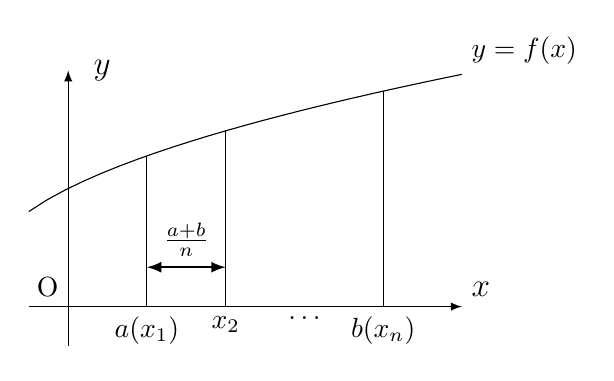
\begin{tikzpicture}
      \path[draw,->,>=latex] (-0.5, 0) -- (5,0) node[above right] {\large $x$};
      \path[draw,->,>=latex] (0, -0.5) -- (0,3) node[right=2mm] {\large $y$} ;
      \path (0,0) node[above left] {$\mathrm{O}$};
      \path[draw,domain=-0.5:5] plot (\x, {sqrt(\x+1)+0.5}) node[above right] {$y=f(x)$};
      \draw [draw] (1,{sqrt(1+1)+0.5}) -- (1,0)node [below] {$a(x_1)$};
      \draw [draw] (2,{sqrt(2+1)+0.5}) -- (2,0)node [below] {$x_2$};
      \draw [draw] (3,0) -- (3,0)node [below] {$\dots$};
      \draw [draw] (4,{sqrt(4+1)+0.5}) -- (4,0)node [below] {$b(x_n)$};
      \draw [thick,latex-latex] (1,0.5) -- (2,0.5) node [above, midway] {$\frac{a+b}{n}$};
\end{tikzpicture}
\caption{合成台形公式のイメージ} 
\label{gtrap}
\end{figure}

表\ref{TrapezoidalRuletable}にTrapezoidalRule関数の機能,引数,返り値の3つを示す.TrapezoidalRule関数は
2点$a$,$b$を$n$分割したときの台形公式による数値積分を求める関数であるから,2点$a$,$b$および分割数$n$を引数,
数値積分の結果を返り値とする設計になっている.

\begin{table}[H]
  \caption{TrapezoidalRule関数の機能,引数,返り値}
  \label{TrapezoidalRuletable}
  \begin{center}
      \begin{tabular}{c|l}\hline
    機能 & 2点$a$,$b$を$n$分割したときの台形公式による数値積分を返す.\\
    引数 & double a,double b,int n\\
    返り値 & double型 \\ \hline
      \end{tabular}
  \end{center}
  \end{table}

  リスト\ref{TrapezoidalRule}にTrapezoidalRule関数のソースコードを示す.リスト\ref{TrapezoidalRule}の2~5行目では分割数$n$が
  不正な値(0や負)である場合にエラーを表示してプログラムを終了する処理を行ってる.ただし,exit関数を用いるためにはstdlib.hをincludeする必要が
  ある.そして,リスト\ref{TrapezoidalRule}の7~11行目では区間[$a$,$b$]を$n$分割して,各区間にTrapezoidal関数を実行する処理を行っている.
  結果はdouble型の引数sumに格納され,returnされる.
      \begin{lstlisting}[basicstyle=\ttfamily\footnotesize, frame=single,label=TrapezoidalRule,caption=TrapezoidalRule関数]
double TrapezoidalRule(double a,double b,int n){
    if(n<=0){
        printf("Incorrect value of n");
        exit(0);
    }

    double sum=0;
    for(double i=0;i<n;i++){
        sum+=Trapezoidal(a+i*(b/n),a+(i+1)*(b/n));
    }
    return sum;
}
            \end{lstlisting}

    \subsubsection{main関数}
    TrapezoidalRule関数を実行し,結果を表示する関数としてmain関数を作成する.リスト\ref{main1}にmain関数のソースコードを示す.
    リスト\ref{main1}の2行目では分割数を1,2,4,$\dots$と細かくするときの上限を定義している.リスト\ref{main1}では
    分割数の上限を256にしている.そして,リスト\ref{main1}の3行目では解析解を定義している.\\
     リスト\ref{main1}の5~11行目では分割数1,2,4,$\dots$,n\_maxについてTrapezoidalRule関数を用いて数学関数$f(x)$の数値積分を
    行い,結果および解析解との誤差の絶対値を表示している.またコメントアウトしている10行目はCSV形式で計算結果を出力するための
    フォーマットである.
      \begin{lstlisting}[basicstyle=\ttfamily\footnotesize, frame=single,label=main1,caption=main1関数]
int main(int argc,char *argv[]){
    int n_max = 256;
    double ans = logf(3)/2;

    double result;
    for(int i=1;i<=n_max;i*=2){
        result = TrapezoidalRule(0,M_PI/6,i);
        printf("n =  %4d  result = %lf  error = %lf\n",i,result,fabs(result-ans));
        // output format for csv
        //printf("%d,%lf,%0.15lf\n",i,result,fabs(result-ans));
    }
    return 0;
}
            \end{lstlisting}

    \subsection{実行結果}
    図\ref{result1}に課題1のプログラムの実行結果を示す.TrapezoidalRule関数による数値積分の結果は
    解析解$\frac{1}{2} \log_{e} 3 = 0.5493061$に十分近い値であることがわかる.注意として,分割数が256のとき
    誤差が0になって完璧な数値解が得られたと思うかもしれないが,これは表示の問題であり実際には表示されている桁より
    も下の桁で誤差が存在している.解析解に収束する様子や誤差の考察については次節で行う.
    
    \begin{figure}[H]
      \centering
      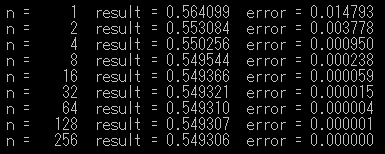
\includegraphics[scale=0.9]{kadai1.png}
      \caption{課題1の実行結果}
       \label{result1}
      \end{figure}

    \subsection{考察}
    分割数を変化させたときの収束の様子や誤差について考察を行う.
    図\ref{fig1-1}に分割数を変化させたときの数値解の収束の様子を示す.ただし分割数は対数軸になっている.
    図\ref{fig1-1}から分割数を大きくする,すなわち刻み幅を細かくすると数値解が解析解に近づく,つまり誤差が減少していることがわかる.
    \begin{figure}[H]
      \centering
      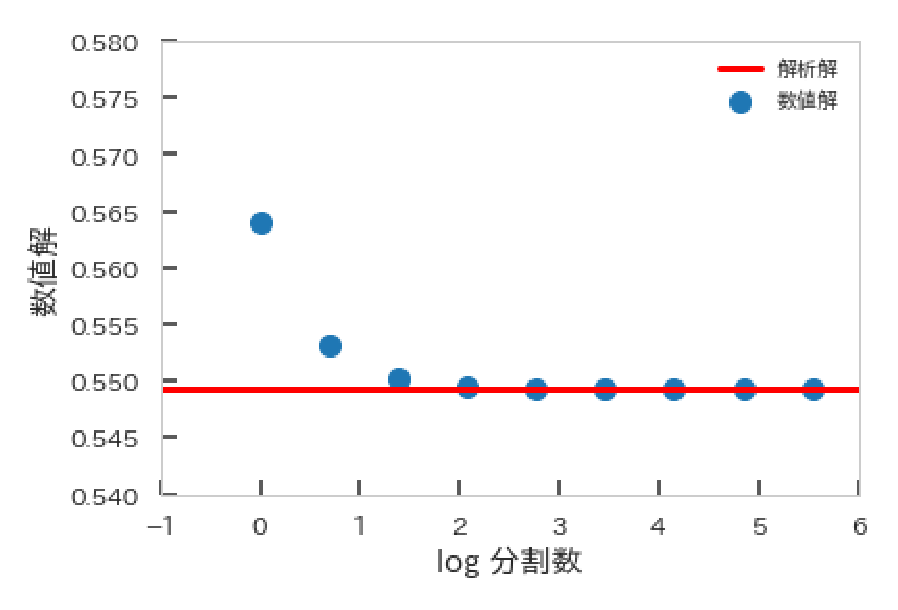
\includegraphics[scale=0.7]{kadai1.eps}
      \caption{数値解の収束の様子(台形公式)}
       \label{fig1-1}
      \end{figure}
      「わかりやすい数値計算入門」!によれば合成台形公式の誤差は$\mathcal{O}(h^2)$である.$\mathcal{O}(h^2)$とは
      分割数$h^2$が2倍になると,精度が4倍になることを意味している.この実験では分割数を$2$倍ずつ
      大きくしているから,1つ前の分割数よりも精度が4倍よくなると予想できる.\\
       表\ref{error1}に1つ前の分割数と比較したときの精度の差を示す.分割数を2倍にすると1つ前の分割数と比較して,精度が平均4.01倍よくなっている.
      このことから分割数$h^2$が2倍になると,精度が4倍になるという予想が正しいことがわかる.
      \begin{table}[H]
        \caption{分割数を大きくしたときの誤差の変化}
      \label{error1}
      \begin{center}
          \begin{tabular}{c|l|r|c}\hline
            分割数 & 数値解 & 誤差 & 1つ前との精度の違い(倍) \\ \hline \hline
            1 & 0.564099 & 0.014793128 & - \\
            2 & 0.553084 & 0.003778157 & 3.92 \\
            4 & 0.550256 & 0.000950031 & 3.98 \\
            8 & 0.549544 & 0.000237854 & 3.99 \\
            16 & 0.549366 & 5.94782E-05 & 4.00 \\
            32 & 0.549321 & 1.48635E-05 & 4.00 \\
            64 & 0.54931 & 3.70853E-06 & 4.01 \\
            128 & 0.549307 & 9.197E-07 & 4.03 \\
            256 & 0.549306 & 2.22487E-07 & 4.13 \\ \hline 
          \end{tabular}
      \end{center}
      \end{table}
       このように,分割数を大きくしたことによって近似の度合いが増加することで減少する誤差を打ち切り誤差という.
      打ち切り誤差はコンピュータ内部の数値の扱いによって生じるものではなく,アルゴリズムの近似精度によって生じる誤差である.
      台形公式では元の数学関数$f(x)$を台形,つまり一次式で近似しているため,分割数が少ない場合は近似精度が十分ではないと
      考えられる.このため,打ち切り誤差が生じる.\\
       打ち切り誤差は分割数を大きくして減少するのであれば,可能な限り分割数を大きくすれば,より正確な数値解を得られる
      と考えられるが,分割数を過剰に大きくすると打ち切り誤差とは別に,丸め誤差の問題が生じる.丸め誤差とは小数点を含む10進数と
      2進数の変換時に生じる誤差である.例えば,10進数の0.6は2進数で表すと0.100110011$\dots$というように無限の桁数が必要である.
      しかしコンピュータで無限の桁数を扱うことはできないのでどこかで桁を丸める必要がある.8ビット目で丸めた場合,
      0.10011001となり,これを10進数に戻すと0.59765626となり元の0.6と誤差が生じる.これが丸め誤差である.\\
       これとは別の誤差の要因として桁落ちが考えられる.桁落ちとは非常に近い値どうしの引き算を行ったときに
      有効数字が急激に減少するために生じる誤差のことである.計算結果の正規化を行う場合,有効桁に0が詰められる
      わけではない.したがって,正規化の結果,有効桁に詰められた0でない数字が目立ってしまう.これが桁落ちによって生じる誤差である.\\
       台形公式の近似(式(\ref{simpleTrapezaidal}))で桁落ちを考慮しなければいけない部分は$b-a$の部分である.
      刻み幅$h$を小さくするとTrapezoidalRule関数で反復的に呼び出す積分区間[$x_i$,$x_{i+1}$]は非常に近い値を持つ.
      このため,$x_{i+1}-x_i$の計算において桁落ちが起きる可能性が考えられる.





    \section{課題2}
    本章では課題2における課題内容,プログラムの説明,実験結果,考察の4つについて述べる.
    \subsection{課題内容}
    課題2の課題内容はシンプソンの公式を用いて式(\ref{kadai2siki})の数値積分を行うものである.
    解析解は$1$である.
    \begin{equation}
      \int_0^\frac{\pi}{2} \sin x dx
          \label{kadai2siki}
        \end{equation}
    数値積分は次の2点についてプログラムの作成および実行を行い結果を考察する.
    \begin{enumerate}
      \item float型とdouble型のそれぞれで数値積分を行い丸め誤差が現れる刻み幅$h$.
      \item 刻み幅を$\frac{1}{2}$倍ずつ変化させたときの誤差の減少.
      \end{enumerate}

    \subsection{プログラムの説明}
    本節では課題2で作成したプログラムにおいて,次に示す4つの関数の役割
    および機能について説明する.なお,課題2ではdouble型およびfloat型のそれぞれで
    数値積分を行う関数を作成したが,ここではdouble型のプログラムのみ説明する.float
    型のプログラムについては,doubleの部分をfloatに変更すれば問題なく実行できる.
    \begin{enumerate}
      \item func関数
      \item Simpson関数
      \item SimpsonRule関数
      \item main関数
      \end{enumerate}
    
    \subsubsection{func関数}
    func関数は課題1と同様に数値計算を行う数学関数を定義する関数である.
    したがって関数の機能,引数,返り値は表\ref{func1table}と同じである.\\
      リスト\ref{func2}にfunc関数のソースコードを示す.func関数は引数xについて積分を行う数学関数$f(x)=\sin x$
      の値を返す.
      \begin{lstlisting}[basicstyle=\ttfamily\footnotesize, frame=single,label=func2,caption=func関数]
double func(double x){
    return sin(x);
} 
            \end{lstlisting}

    \subsubsection{Simpson関数}
    Simpson関数は数学関数$f(x)$において与えられた2点$a$,$b$におけるシンプソン法による数値積分を行う関数である.
    $a$から$b$までの$f(x)$の積分はシンプソン法により式(\ref{simpleSimpson})のように近似できる.ただし,$h$は積分を行う
    区間の幅である.すなわち$h=\frac{b-a}{2}$である.
    \begin{equation}
      \int_a^b f(x) dx \simeq \frac{h}{3} \left[ f(a)+4f \left( \frac{a+b}{2} \right) +f(b) \right] 
          \label{simpleSimpson}
        \end{equation}
     式(\ref{simpleSimpson})の意味について説明する.台形公式では2点$a$,$b$のおける$f(a)$,$f(b)$の値のみを用いて数値積分
    を行っていた(式(\ref{simpleTrapezaidal}))がさらに精度を高めたい.そこで$a$,$b$の中点$\frac{a+b}{2}$の値を用いて2
    次の近似を行う.3点における$f(x)$の値をそれぞれ$y_0,y_1,y_2$とする.このとき,$\frac{h}{2}$を基準とすると,3点は$(-h,y_0),(0,y_1),(h,y_2)$
    と表せる.$f(x)$を近似する2次多項式$y=a+bx+cx^2$とおくと式(\ref{startr})~式(\ref{endr})の連立方程式が得られる.
    \begin{numcases}
      {}
      \label{startr}
      a-bh+ch^2= y_0 & \\
      a = y_0 & \\
      \label{betweenr}
      a+bh+ch^2=y_2
      \label{endr} 
    \end{numcases}
      式(\ref{startr})$+$式(\ref{betweenr})$\times 4$+式(\ref{endr})を計算すると式(\ref{forsimp})が得られる.これを
      面積$S$の計算に用いることでシンプソン法の式(\ref{simpleSimpson})が得られる.
    \begin{eqnarray}
      (a-bh+ch^2)+4a+(a+bh+ch^2) &=& y_0 +4y_1+y_2 \\
      6a+2ch^2 &=& y_0 +4y_1+y_2 
      \label{forsimp}
    \end{eqnarray}
     求めたい面積$S$を2次多項式の近似で計算すると式(\ref{forsimp2})のようにシンプソン法の式(\ref{simpleSimpson})
    が得られる.式(\ref{forsimp2})の計算において,式(\ref{tmp1})から式(\ref{forsimp2})の計算には式(\ref{forsimp})
    を用いている.

    \begin{eqnarray}
      S &=& \int_{-h}^{h} (a+bx+cx^2) dx \\
      &=& 2 \int_{0}^{h} (a+cx^2) dx \\
      &=& 2 \left[ ax+\frac{cx^3}{3} \right]_0^h \\
      &=& \frac{h}{3}(6a+2ch^2) \label{tmp1}\\
      &=& \frac{h}{3} \left[ f(a)+4f \left( \frac{a+b}{2} \right) +f(b) \right] 
      \label{forsimp2}
    \end{eqnarray}
    
    表\ref{Simpsontable}にSimpson関数の機能,引数,返り値の3つを示す.Simpson関数は2点$a$,$b$における
    シンプソン法による数値積分を行う関数であるから,2点$a$,$b$を引数,数値積分の結果を返り値とする設計になっている.
    \begin{table}[H]
      \caption{Simpson関数の機能,引数,返り値}
      \label{SimpsonTtable}
      \begin{center}
          \begin{tabular}{c|l}\hline
        機能 & 2点$a$,$b$におけるシンプソン法による数値積分を返す.\\
        引数 & double a,double b\\
        返り値 & double型 \\ \hline
          \end{tabular}
      \end{center}
      \end{table}

      リスト\ref{Simpson}にSimpson関数のソースコードを示す.Simpson関数は引数$a$,$b$について式(\ref{simpleSimpson})
      の計算結果を返す.
      \begin{lstlisting}[basicstyle=\ttfamily\footnotesize, frame=single,label=Simpson,caption=Simpson関数]
double Simpson(double a,double b){
    double h = (b-a)/2;
    double c = (a+b)/2;
    return h*(func(a)+4*func(c)+func(b))/3;
}
      \end{lstlisting}

    \subsubsection{SimpsonRule関数}
    SimpsonRule関数は区間[$a$,$b$]を$n$個に分割して,分割した区間のそれぞれにシンプソン法による数値積分を適用する関数である.
    区間を分割して積分を行うイメージとしてはTrapezoidalRule関数と同様である.\\
     表\ref{SimpsonRuleTtable}にSimpsonRule関数の機能,引数,返り値の3つを示す.SimpsonRule関数は
    2点$a$,$b$を$n$分割したときのシンプソン法による数値積分を求める関数であるから,2点$a$,$b$および分割数$n$を引数,
    数値積分の結果を返り値とする設計になっている.

    \begin{table}[H]
      \caption{SimpsonRule関数の機能,引数,返り値}
      \label{SimpsonRuleTtable}
      \begin{center}
          \begin{tabular}{c|l}\hline
        機能 & 2点$a$,$b$を$n$分割したときのシンプソン法による数値積分を返す.\\
        引数 & double a,double b,int n\\
        返り値 & double型 \\ \hline
          \end{tabular}
      \end{center}
      \end{table}

      リスト\ref{SimpsonRule}にSimpsonRule関数のソースコードを示す.
      リスト\ref{SimpsonRule}の2~5行目では分割数$n$が不正な値(0や負)である場合にエラーを表示してプログラムを終了する処理を行ってる.
      そして,リスト\ref{SimpsonRule}の6~11行目では区間[$a$,$b$]を$n$分割して,各区間にSimpson関数を実行する処理を行っている.結果はdouble型の引数sumに格納され,returnされる.
      \begin{lstlisting}[basicstyle=\ttfamily\footnotesize, frame=single,label=SimpsonRule,caption=SimpsonRule関数]
double SimpsonRule(double a,double b,int n){
    if(n<=0){
        printf("Incorrect value of n");
        exit(0);
    }
    double sum=0;
    for(double i=0;i<n;i++){
        sum+=Simpson(a+i*(b/n),a+(i+1)*(b/n));
    }
    return sum;
}
            \end{lstlisting}

    \subsubsection{main関数}
    SimpsonRule関数を実行し,結果を表示する関数としてmain関数を作成する.リスト\ref{main2}にmain関数のソースコードを示す.
    リスト\ref{main2}の2行目では分割数を1,2,4,$\dots$と細かくするときの上限を定義している.リスト\ref{main2}では
    分割数の上限を256にしている.
     リスト\ref{main2}の3~7行目では分割数1,2,4,$\dots$,n\_maxについてSimpsonlRule関数を用いて数学関数$f(x)$の数値積分を
    行い,結果(少数以下16桁)および解析解との誤差の絶対値を表示している.ただし解析解3.141592はオブジェクト形式マクロで定義している.
      \begin{lstlisting}[basicstyle=\ttfamily\footnotesize, frame=single,label=main2,caption=main2関数]
int main(int argc,char *argv[]){
    int n_max = 256;
    for(int i=1; i<=n_max; i*=2){
        double result = SimpsonRule(0,M_PI/2,i);
        printf("split = %4d   result = %1.16lf   error = %1.16lf\n",
        i,result,fabs((double)1-result));
    }
    return 0;
}
    \end{lstlisting}

    \subsection{実行結果}
    図\ref{kadai2d}に課題2のプログラムのdouble型における実行結果,図\ref{kadai2f}にfloat型における実行結果を示す.
    float型では256分割,double型では65536分割まで実行した.図\ref{kadai2d}および図\ref{kadai2f}において,分割数1から256についてSimpsonRule関数を実行できていることがわかる.
    どちらの実行結果においても数値積分の結果が1に収束していることが読み取れる.解析解に収束する様子や誤差の考察は次節で行う.
    \begin{figure}[H]
      \centering
      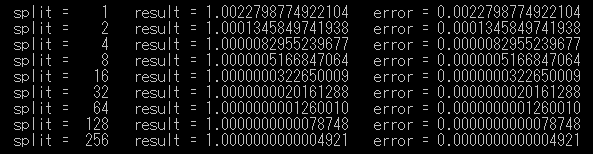
\includegraphics[scale=0.9]{kadai2double.png}
      \caption{課題2の実行結果(double型)}
       \label{kadai2d}
      \end{figure}

      \begin{figure}[H]
        \centering
        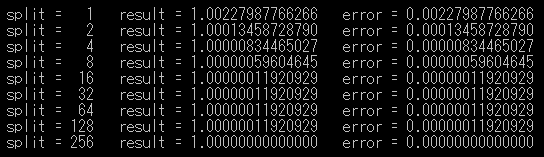
\includegraphics[scale=0.9]{kadai2float.png}
        \caption{課題2の実行結果(float型)}
         \label{kadai2f}
        \end{figure}

    \subsection{考察}
    本節では次に示す2つの考察について述べる.
    \subsubsection{丸め誤差の現れる刻み幅$h$}
    丸め誤差とは有限桁の2進数で表せない数値を丸めるさいに発生する誤差であった.IEEE754によればfloat型,double型の
    内部表現は次のようになっている.
    \begin{itemize}
      \item float型(32ビット)$\dots$符号部1ビット,指数部8ビット,仮数部23ビット
      \item double型(64ビット)$\dots$符号部1ビット,指数部11ビット,仮数部52ビット
    \end{itemize}
     float型の精度は10進数で7桁,double型では15桁である.すなわち丸め誤差はfloat型では7桁目,double型では15桁目
    付近で現れるはずである.\\
     実行結果で実際の丸め誤差を確認する.まずdouble型について確認する.double型の実行結果(図\ref{kadai2d})は小数点以下16桁を表示している.
    分割数が4096のとき,小数点以下15桁に0がたっており,16桁目に7がたっている.さらに,4096より分割数を大きくしても,数値解が収束していないことが読み取れる.
    このことから,分割数が4096のときにdouble型の丸め誤差が生じると考えられる.これよりも精度が必要な場合は多倍長演算を行う必要がある.\\
     次にfloat型について確認する.float型の実行結果(図\ref{kadai2f})は小数点以下16桁を表示している.
    分割数が16のとき,小数点以下6桁に0がたっており,7桁目に1がたっている.さらに,分割数が16から128のとき,数値解がすべて一致している.
    これらを踏まえると,分割数が16のときにfloat型の丸め誤差が生じると考えられる.

    \subsubsection{刻み幅を$\frac{1}{2}$ずつ変化させたときの誤差の減少}

    \section{課題3~5}
    本章では課題3~5の課題内容,プログラムの説明,実行結果,考察について述べる.
    \subsection{課題内容}
    課題3~5では式(\ref{kadai3siki})に示す微分方程式を3つのアルゴリズムで解き,誤差および精度について考察する.
    ただし式(\ref{kadai3siki})の初期条件は$u(0)=1$である.式(\ref{kadai3siki})の解析解は$e^t$である.
    課題3ではオイラー法,課題4ではホイン法,課題5ではルンゲ・クッタ法で微分方程式を解く.
      \begin{equation}
      \frac{du}{dt} = u
          \label{kadai3siki}
        \end{equation}

    \subsection{プログラムの説明}
    本節では課題3~5で作成したプログラムにおいて,次に示す5つの関数の役割
    および機能について説明する.
    \begin{enumerate}
      \item func関数
      \item Euler関数
      \item Heun関数
      \item RK関数
      \item main関数
      \end{enumerate}

      \subsubsection{func関数}
      func関数は式(\ref{funcsiki3})に示すように微分方程式の右辺の数学関数を定義する関数である.
      \begin{equation}
        \frac{dy}{dx} = f(x,y)
            \label{funcsiki3}
          \end{equation}

      表\ref{func3table}にfunc関数の機能,引数,返り値の3つを示す.
    func関数は数学関数を定義する関数であるから,引数$x$,$y$(double型)について返り値$f(x,y)$を返す設計になっている.

      \begin{table}[H]
      \caption{func関数の機能,引数,返り値}
      \label{func3table}
      \begin{center}
          \begin{tabular}{c|l}\hline
        機能 & 数学関数を定義する\\
        引数 & double x,double y \\
        返り値 & double型 \\ \hline
          \end{tabular}
      \end{center}
      \end{table}
      リスト\ref{func3}にfunc関数のソースコードを示す.func関数は引数$x$,$y$について微分方程式の右辺の数学関数$f(x) = y$の値を
      返す.
      \begin{lstlisting}[basicstyle=\ttfamily\footnotesize, frame=single,label=func3,caption=func関数]
double func(double x,double y){
    return y;
}
      \end{lstlisting}
      
      \subsubsection{Euler関数}
      課題3のプログラムとして微分方程式をEuler法で解く関数としてEuler関数を作成する.今与えられている微分方程式の情報は
      式(\ref{funcsiki3})および初期条件である.この情報のみから,解析的手法を用いずに数値解を求める方法を考える.\\
       コンピュータでは無限に小さい値を扱うことができないから式(\ref{funcsiki3})を式(\ref{funcsikikinji})のように
      近似する.$\frac{\Delta y}{\Delta x}$は十分小さい値という意味合いだと思ってもらいたい.
      \begin{eqnarray}
        \frac{dy}{dx} \approx \frac{\Delta y}{\Delta x} = f(x,y)
            \label{funcsikikinji}
      \end{eqnarray}

      式(\ref{funcsikikinji})を変形すると式(\ref{henkei})のようになる.
      \begin{eqnarray}
        \Delta y = f(x,y)\Delta x
            \label{henkei}
      \end{eqnarray}
    
      $\Delta y=y_1-y_0$,$\Delta x=x_1-x_0$,$h=x_1-x_0$とすると,式(\ref{henkei})は
      式(\ref{henkei2})のように変形できる.
      \begin{eqnarray}
        y_1 -y_0 &=& h f(x_0,y_0) 
            \label{henkei2}
      \end{eqnarray}
      これを一般化すると,式(\ref{eulersiki1})および式(\ref{eulersiki2})に示すように$x_{i+1}$,$y_{i+1}$を反復的に計算することによって数値解を求めることができる.
      これをEuler法という.Euler関数は式(\ref{eulersiki2})の計算を反復的に行う関数である.
      \begin{eqnarray}
        x_{i+1} &=& x_i+h \label{eulersiki1}\\
        y_{i+1} &=& y_i + hf(x_i,y_i)
            \label{eulersiki2}
      \end{eqnarray}

      表\ref{Eulertable}にEuler関数の機能,引数,返り値の3つを示す.
      Euler関数はEuler法による微分方程式の数値解を求める関数であるから,初期条件$x_0,y_0$および刻み幅$h$を引数とする
      設計になっている.結果は標準出力を行うため返り値はない.
  
        \begin{table}[H]
        \caption{Euler関数の機能,引数,返り値}
        \label{Eulertable}
        \begin{center}
            \begin{tabular}{c|l}\hline
          機能 & 式(\ref{eulersiki2})を反復的に計算し,結果を標準出力に表示する.\\
          引数 & double x0,double y0,double h \\
          返り値 & なし(void) \\ \hline
            \end{tabular}
        \end{center}
        \end{table}

        リスト\ref{Euler}にEuler関数のソースコードを示す.リスト\ref{Euler}の4行目から10行目が式(\ref{eulersiki2})を
        反復的に計算する部分である.ただしループ回数の上限はオブジェクト形式マクロでMAX\_STEPという値を宣言する必要がある.
      \begin{lstlisting}[basicstyle=\ttfamily\footnotesize, frame=single,label=Euler,caption=Euler関数]
void Euler(double x0,double y0,double h){
    double x=x0,y=y0;
    double xp,yp;
    for(int i=0;i<MAX_STEP;i++){
        xp = x+h;
        yp = y+h*func(x,y);
        printf("t=%02d   x=%lf,y=%lf\n",i+1,xp,yp);
        x=xp;
        y=yp;
    }
}
      \end{lstlisting}

      \subsubsection{Heun関数}
      課題4のプログラムとして微分方程式をHeun法で解く関数であるHeun関数を作成する.Heun法は
      Euler法を改善し,精度を向上させた方法である.式(\ref{Heunsiki})にHeun法の計算式を示す.
      Euler法では$f(x_i,y_i)$のみを用いて数値解を求めたが,Heun法では$f(x_i,y_i)$と$f(x_i+h,y_i+hf(x_i,y_i))$
      の平均を用いて数値解を計算している.
      \begin{eqnarray}
        x_{i+1} &=& x_i+h \label{eulersiki1}\\
        k_1 &=& hf(x_i,y_i)\\
        k_2 &=& h(x_i+h,y_i+k_1) \\
        y_{i+1} &=& y_i + \frac{1}{2}(k_1+k_2)
            \label{Heunsiki}
      \end{eqnarray}

      Heun関数は,Euler関数と微分方程式を数値解で求める内部のアルゴリズムが異なるだけである.このため,関数設計(引数,返り値)は表\ref{Eulertable}と同じである.\\
       リスト\ref{Heun}にHeun関数のソースコードを示す.リスト\ref{Heun}の4行目から11行目が反復的に式(\ref{Heunsiki})を計算している部分である.
    \begin{lstlisting}[basicstyle=\ttfamily\footnotesize, frame=single,label=Heun,caption=Heun関数]
void Heun(double x0,double y0,double h){
    double x=x0,y=y0;
    double xp,yp,k1,k2;
    for(int i=0;i<MAX_STEP;i++){
        xp = x+h;
        k1 = h*func(x,y);
        k2 = h*func(x+h,y+k1);
        yp = y+(k1+k2)/2;
        printf("t=%02d   x=%lf,y=%lf\n",i+1,xp,yp);
        x=xp;
        y=yp;
    }
}
    \end{lstlisting}      
      
      \subsubsection{RK関数}
      課題5のプログラムとして微分方程式をルンゲ・クッタ法で解く関数であるRK関数を作成する.ルンゲ・クッタ法は
      一般に微分方程式の数値解を求めるのに用いられる4次近似の方法である.Heun法で2次近似を行ったものと考え方は
      同じである.式(\ref{RKsiki})にルンゲ・クッタ法の計算式を示す.式(\ref{RKsiki})において,$k_2$,$k_3$は
      2倍の重みで扱われている.
      \begin{eqnarray}
        x_{i+1} &=& x_i+h \label{eulersiki1}\\
        k_1 &=& hf(x_i,y_i)\\
        k_2 &=& h(x_i+\frac{h}{2},y_i+\frac{k_1}{2}) \\
        k_3 &=& h(x_i+\frac{h}{2},y_i+\frac{k_2}{2}) \\
        k_4 &=& hf(x_i+h,y_i+k_3)\\
        y_{i+1} &=& y_i +\frac{1}{6}(k_1+2k_2+2k_3+k_4)
            \label{RKsiki}
      \end{eqnarray}

      RK関数の関数設計もEuler関数,Heun関数の内部のアルゴリズムが異なるだけであるから,表\ref{Eulertable}と同じである.\\
       リスト\ref{RK}にHeun関数のソースコードを示す.リスト\ref{RK}の4行目から20行目が反復的に式(\ref{RKsiki})を計算している部分である.
    \begin{lstlisting}[basicstyle=\ttfamily\footnotesize, frame=single,label=RK,caption=RK関数]
void RK(double x0,double y0,double h){
    double x=x0,y=y0;
    double xp,yp,k1,k2,k3,k4;
    for(int i=0;i<MAX_STEP;i++){
        xp = x+h;
        k1 = h*func(x,y);
        k2 = h*func(x+h/2,y+k1/2);
        k3 = h*func(x+h/2,y+k2/2);
        k4 = h*func(x+h,y+k3);
        yp = y+(k1+2*k2+2*k3+k4)/6;
        printf("t=%02d   x=%lf,y=%lf\n",i+1,xp,yp);
        /* print k1,k2,k3,k4
        printf("k1=%lf\n",k1);
        printf("k2=%lf\n",k2);
        printf("k3=%lf\n",k3);
        printf("k4=%lf\n",k4);
        */
        x=xp;
        y=yp;
    }
}

    \end{lstlisting}   
      \subsubsection{main関数}
      Euler関数,Heun関数,RK関数を実行する関数としてメイン関数を作成する.リスト\ref{main3}にmain関数のソースコードを示す.
      リスト\ref{main3}では,初期条件および刻み幅$h$の定義をしている.そして6行目から14行目でEuler関数,Heun関数,RK関数を
      実行している.
      \begin{lstlisting}[basicstyle=\ttfamily\footnotesize, frame=single,label=main3,caption=main関数]
int main(int argc,char *argv[]){
    double x0 = 0;
    double y0 = 1;
    double h = 0.1;

    /* format for stdout*/
    printf("-----setting-----\n");
    printf("h=%lf\nt=00   x=%lf,y=%lf\n",h,x0,y0);
    printf("\n-----Euler method-----\n");
    Euler(x0,y0,h);
    printf("\n-----Heun method-----\n");
    Heun(x0,y0,h);
    printf("\n-----Runge-kutta method-----\n");
    RK(x0,y0,h);
    
    return 0;
}
            \end{lstlisting}      

    \subsection{実行結果}
    表\ref{h01}~表\ref{h005}に刻み幅$h$を次に示す3つの値に変化させたときの実行結果を示す.
    \begin{enumerate}
      \item MAX\_STEP = 10,$h$=0.1
      \item MAX\_STEP = 2,$h$=0.5
      \item MAX\_STEP = 20,$h$=0.05
    \end{enumerate}

    \begin{table}[H]
      \caption{MAX\_STEP = 10,$h$=0.1のときの実行結果}
    \label{h01}
    \begin{center}
        \begin{tabular}{r|c|l|l|l}\hline
          $step$ & $t$ & $u$(Euler) & $u$(Heun) & $u$(RK) \\ \hline \hline
0 & 0 & 1 & 1 & 1 \\ 
1 & 0.1 & 1.1 & 1.105 & 1.105171 \\ 
2 & 0.2 & 1.21 & 1.221025 & 1.221403 \\ 
3 & 0.3 & 1.331 & 1.349233 & 1.349858 \\ 
4 & 0.4 & 1.4641 & 1.490902 & 1.491824 \\ 
5 & 0.5 & 1.61051 & 1.647447 & 1.648721 \\ 
6 & 0.6 & 1.771561 & 1.820429 & 1.822118 \\ 
7 & 0.7 & 1.948717 & 2.011574 & 2.013752 \\ 
8 & 0.8 & 2.143589 & 2.222789 & 2.22554 \\ 
9 & 0.9 & 2.357948 & 2.456182 & 2.459601 \\ 
10 & 1 & 2.593742 & 2.714081 & 2.71828 \\ \hline
        \end{tabular}
    \end{center}
    \end{table}

        \begin{table}[H]
      \caption{MAX\_STEP = 2,$h$=0.5のときの実行結果}
    \label{h05}
    \begin{center}
        \begin{tabular}{r|c|l|l|l}\hline
          $step$ & $t$ & $u$(Euler) & $u$(Heun) & $u$(RK) \\ \hline \hline
          0 & 0 & 1 & 1 & 1 \\
          1 & 0.5 & 1.5 & 1.625 & 1.648438 \\ 
          2 & 1 & 2.25 & 2.640625 & 2.717346 \\ \hline
        \end{tabular}
    \end{center}
    \end{table}

    \begin{table}[H]
      \caption{MAX\_STEP = 20,$h$=0.05のときの実行結果}
    \label{h005}
    \begin{center}
        \begin{tabular}{r|c|l|l|l}\hline
          $step$ & $t$ & $u$(Euler) & $u$(Heun) & $u$(RK) \\ \hline \hline
          0 & 0 & 1 & 1 & 1 \\
          1 & 0.05 & 1.05 & 1.05125 & 1.051271 \\
          2 & 0.1 & 1.1025 & 1.105127 & 1.105171 \\
          3 & 0.15 & 1.157625 & 1.161764 & 1.161834 \\
          4 & 0.2 & 1.215506 & 1.221305 & 1.221403 \\
          5 & 0.25 & 1.276282 & 1.283897 & 1.284025 \\
          6 & 0.3 & 1.340096 & 1.349696 & 1.349859 \\
          7 & 0.35 & 1.4071 & 1.418868 & 1.419068 \\
          8 & 0.4 & 1.477455 & 1.491585 & 1.491825 \\
          9 & 0.45 & 1.551328 & 1.568029 & 1.568312 \\
          10 & 0.5 & 1.628895 & 1.64839 & 1.648721 \\
          11 & 0.55 & 1.710339 & 1.73287 & 1.733253 \\
          12 & 0.6 & 1.795856 & 1.82168 & 1.822119 \\
          13 & 0.65 & 1.885649 & 1.915041 & 1.915541 \\
          14 & 0.7 & 1.979932 & 2.013187 & 2.013753 \\
          15 & 0.75 & 2.078928 & 2.116363 & 2.117 \\
          16 & 0.8 & 2.182875 & 2.224826 & 2.225541 \\
          17 & 0.85 & 2.292018 & 2.338849 & 2.339647 \\
          18 & 0.9 & 2.406619 & 2.458715 & 2.459603 \\
          19 & 0.95 & 2.52695 & 2.584724 & 2.58571 \\
          20 & 1 & 2.653298 & 2.717191 & 2.718282 \\ \hline
        \end{tabular}
    \end{center}
    \end{table}



    \subsection{考察}
    本節では各手法における誤差,精度の様子,および誤差の考察について述べる.
    \subsubsection{誤差,精度の様子}
    各手法について,刻み幅$h$を変化させたときの数値解を考察する.まずEuler法による数値解をプロットしてみる.
    図\ref{eulerplt}に刻み幅$h$を0.1,0.5,0.05にしたときのEuler法の数値解のプロットを示す.$t$が小さいうちは
    どの刻み幅でも誤差が小さいことが読み取れる.一方で$t=1$付近では数値解と解析解の誤差が大きく,
    特に刻み幅$h=0.5$の数値解の誤差大きく目立つことがわかる.$h=0.5,t=1$のときのEuler法の数値解は,表\ref{h05}より
    2.25である.解析解$e=2.7181...$であるから0.468という非常に大きい誤差があることがわかる.一方で最も
    正確な$h=0.05,t=1$のときのEuler法による数値解は,表\ref{h005}より2.653298であることがわかる.
    解析解$e=2.7181...$との誤差は0.065である.同条件でのルンゲ・クッタ法の数値解が2.718282と比較すると
    精度が不十分であることがわかる.

    \begin{figure}[H]
      \centering
      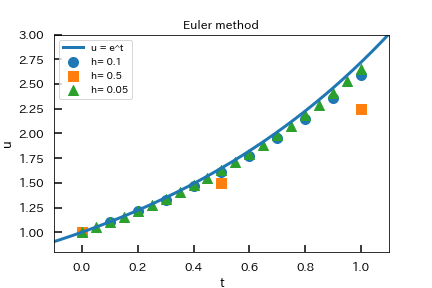
\includegraphics[scale=0.75]{kadai3.png}
      \caption{刻み幅$h$を変化させたときの数値解の様子(Euler法)}
       \label{eulerplt}
      \end{figure}

    次にHeun法による数値解をプロットして,様子を考察する.図\ref{heunplt}に刻み幅$h$を0.1,0.5,0.05にしたときのEuler法の数値解のプロットを示す.
    図\ref{eulerplt}と図\ref{heunplt}を比較するとHeun法のほうがどの刻み幅$h$でも数値解の誤差が小さいことが読み取れる.
    Euler法で誤差が大きかった$h=0.5,t=1$の数値解は表\ref{h05}より2.640625であることが読み取れる.解析解との差は0.078であり
    Euler法と比較すると0.4も精度が上がっていることがわかる.また,$h=0.05,t=1$のときは,表\ref{h005}より数値解は2.717191であることが読み取れる.
    同条件のEuler法と比較すると,0.06精度が上がっていることが読み取れる.これらを踏まえると,Euler法よりも2次の近似を行ったHeun法のほうが精度が
    よいことがわかる.
    \begin{figure}[H]
      \centering
      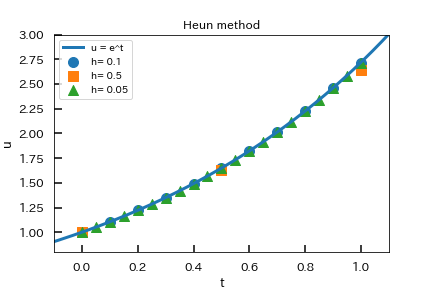
\includegraphics[scale=0.75]{kadai4.png}
      \caption{刻み幅$h$を変化させたときの数値解の様子(Heun法)}
       \label{heunplt}
      \end{figure}

    最後にルンゲ・クッタ法による数値解をプロットして様子を考察する.図\ref{RKplt}に刻み幅$h$を0.1,0.5,0.05にしたときのルンゲ・クッタ法の数値解のプロットを示す.
    図\ref{RKplt}において数値解は解曲線上にのっていることが読み取れる.このことからEuler法,Heun法と比較してルンゲ・クッタ法はより精度が高いことが考えられる.
    実際,$h=0.05,t=1$のときの数値解は2.718282であり,解析解$e=2.7181828...$と小数点以下6桁は一致していることがわかる.
    \begin{figure}[H]
      \centering
      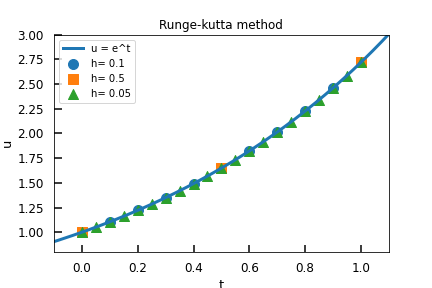
\includegraphics[scale=0.75]{kadai5.png}
      \caption{刻み幅$h$を変化させたときの数値解の様子(ルンゲ・クッタ法)}
       \label{RKplt}
      \end{figure}

    \subsubsection{誤差の考察}
    「わかりやすい数値計算入門」!によればEuler法,Heun法,ルンゲ・クッタ法の誤差のオーダーは表\ref{rkgosa}のようになっている.
    ここで局所離散化誤差とは各ステップで生じる誤差のことであり,大域離散化誤差は局所離散化誤差が蓄積した誤差のことである.
    今考えている誤差は大域離散化誤差である.
    \begin{table}[H]
      \caption{ルンゲ・クッタ型公式の誤差}
    \label{rkgosa}
    \begin{center}
        \begin{tabular}{c|c|c|c}\hline
          公式 & 次数 & 局所誤差 & 大域誤差 \\ \hline \hline
          Euler法 & 1 & $\mathcal{O}(h^2)$ & $\mathcal{O}(h)$ \\ 
          Heun法 & 2 & $\mathcal{O}(h^3)$ & $\mathcal{O}(h^2)$ \\
          ルンゲ・クッタ法 & 4 & $\mathcal{O}(h^5)$ & $\mathcal{O}(h^4)$ \\ \hline
        \end{tabular}
    \end{center}
    \end{table}
    
    大域離散化誤差が表\ref{rkgosa}に従っているか確認する.
    まずEuler法の場合について確認する.この実験では刻み幅$h$を0.5,0.1,0.05のように変化させているから
    刻み幅$h=$0.5の数値解と刻み幅$h=$0.05の数値解では精度に10倍の違いがあり,刻み幅$h$0.1の
    数値解と刻み幅$h$0.05の数値解では精度に2倍の違いがあると予想できる.\\
     表\ref{eulergosa}に$t=0.5$および$t=1$のときの解析解と数値解との誤差を示す.ただし$e^{0.5}=1.6487...$,
    $e=2.7182...$である.表\ref{eulergosa}から刻み幅$h=$0.5の数値解と刻み幅$h=$0.05の数値解では精度は平均7.25倍
    よくなっていることが計算できる.これは理論値である10倍の精度になっているとは言えないが,$\mathcal{O}(h)$から大きく
    外れた精度にはなっていない.
    刻み幅$h=$0.1の数値解と刻み幅$h=$0.05の数値解では精度が平均1.91倍よくなっていることが計算できる.これは理論値である
    2倍に合致した結果である.以上のことからEuler法の大域離散化誤差は$\mathcal{O}(h)$になっていることが確認できたと考える.

    \begin{table}[H]
      \caption{数値解と解析解の誤差(Euler法)}
    \label{eulergosa}
    \begin{center}
        \begin{tabular}{c|c|c|c}\hline 
          & $h=0.5$ & $h=0.1$ & $h=0.05$ \\ \hline \hline 
          $t=0.5$ & 0.149 & 0.038 & 0.020 \\ 
          $t=1.0$ & 0.458 & 0.125 & 0.065 \\ \hline
        \end{tabular}
    \end{center}
    \end{table}    

   次にHeun法の場合について確認する.Heun法の場合も$t=0.5,t=1.0$で検証する.表\ref{heungosa}に$t=0.5$および$t=1$のときの解析解と数値解との誤差を示す.
  Heun法の大域離散化誤差は$\mathcal{O}(h^2)$であるから,刻み幅$h=$0.5の数値解と刻み幅$h=$0.05の数値解では精度に100倍の違いがあり,刻み幅$h$0.1の
  数値解と刻み幅$h$0.05の数値解では精度に4倍の違いがあると予想できる.\\
  表\ref{eulergosa}から刻み幅$h=$0.5の数値解と刻み幅$h=$0.05の数値解では精度は平均71.2倍よくなっていることが計算できる.
  これは理論値である100倍の精度になっているとは言えないが,$\mathcal{O}(h^2)$から大きく外れた精度にはなっていない.
  刻み幅$h=$0.1の数値解と刻み幅$h=$0.05の数値解では精度が平均7.55倍よくなっていることが計算できる.
  これは理論値である4倍の精度になっているとは言えないが,$\mathcal{O}(h)$から大きく外れた精度にはなっていない.
  これらから,理論値の精度には達していないが,Heun法の大域離散化誤差は$\mathcal{O}(h)$になっていることが確認できたと考える.

  \begin{table}[H]
    \caption{数値解と解析解の誤差(heun法)}
  \label{heungosa}
  \begin{center}
      \begin{tabular}{c|c|c|c}\hline 
        & $h=0.5$ & $h=0.1$ & $h=0.05$ \\ \hline \hline 
        $t=0.5$ & 0.02371 & 0.00123 & 0.00033 \\ 
        $t=1.0$ & 0.0777 & 0.0042 & 0.0011 \\ \hline
      \end{tabular}
  \end{center}
  \end{table}    


        \begin{thebibliography}{9}
          \bibitem{NNCT}  伊藤祥一,多倍長演算 3Jアルゴリズムとデータ構造 後期,2019年9月4日
          \end{thebibliography}

\end{document}

